% !TEX TS-program = pdflatex
% !TEX encoding = UTF-8 Unicode

% Matthew Urffer Master Thesis
% 
% Sim Performance
%
\section{Simulation}

%%%%%%%%%%%%%%%%%%%%%%%%%%%%%%%%%%%%%%%%%%%%%%%%%%%%%%%%%%%%%%%%%%%%%%%%%%%%%%%
%                                                                             %
%                                 Single Film                                 %
%                                                                             %
%%%%%%%%%%%%%%%%%%%%%%%%%%%%%%%%%%%%%%%%%%%%%%%%%%%%%%%%%%%%%%%%%%%%%%%%%%%%%%%
\subsection{Single Film}
%%%%%%%%%%%%%%%%%%%%%%%%%%%%%%%%%%%%%%%%%%%%%%%%%%%%%%%%%%%%%%%%%%%%%%%%%%%%%%%
\begin{frame}{Single Film Model}
\begin{columns}[onlytextwidth]
\begin{column}{0.45\textwidth}
\begin{itemize}
	\item Test configuration mocked up in MCNPX
	\item Single film simulated
\end{itemize}
	\tiny
	\begin{figure}
		\centering
		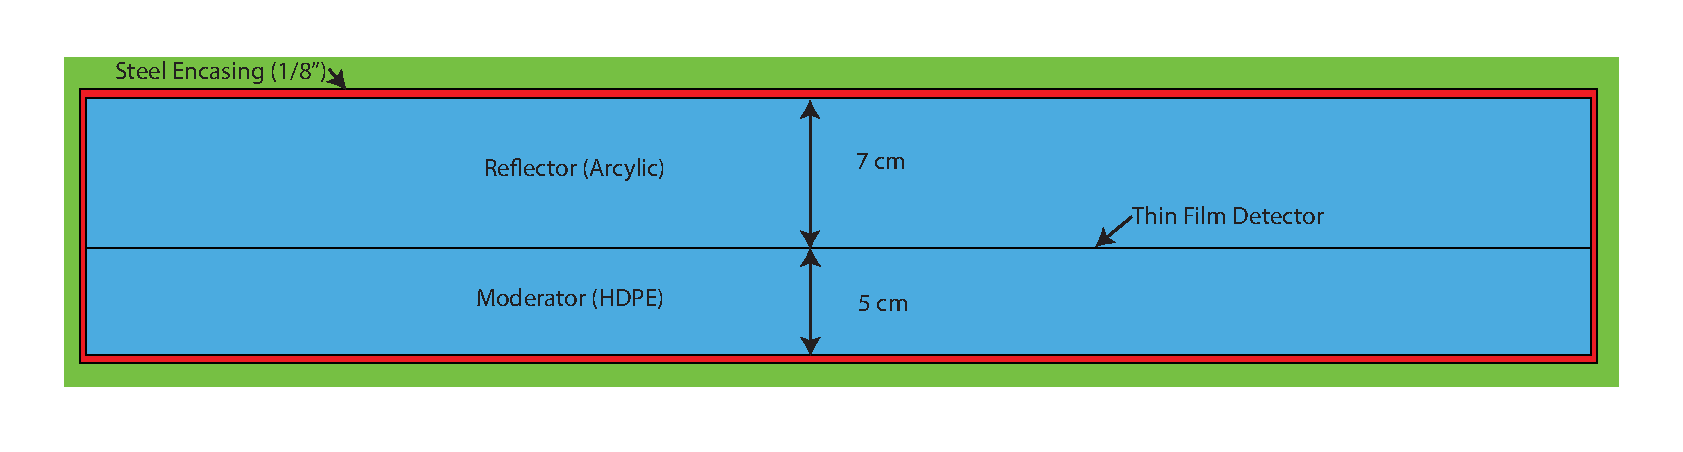
\includegraphics[width=\textwidth]{images/SingleFilm_DetectorAssembly.eps}
		\caption{Simulated RPM8 Detector}
	\end{figure}
\end{column}
\begin{column}{0.45\textwidth}
	\tiny
	\begin{figure}
		\centering
		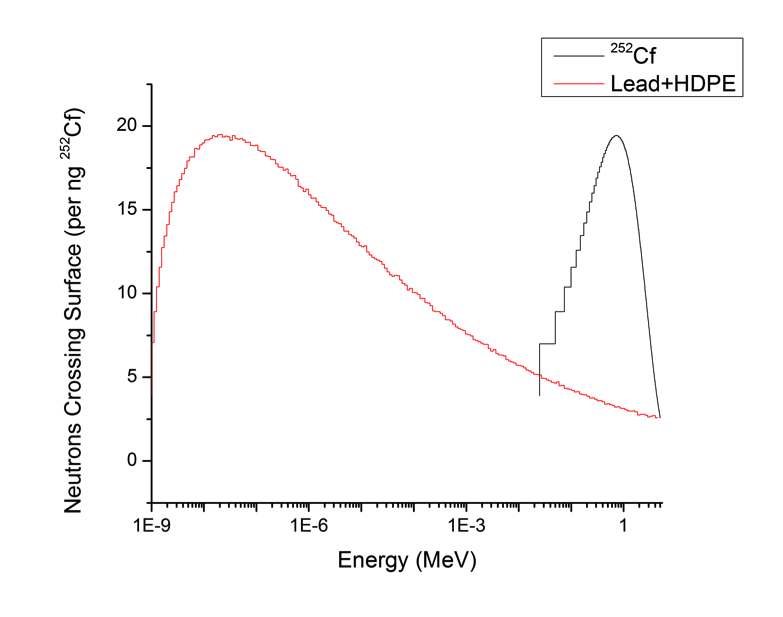
\includegraphics[width=\textwidth]{images/WattFission.eps}
		\caption{Source and incident Spectra}
	\end{figure}
\end{column}
\end{columns}
\end{frame}
%%%%%%%%%%%%%%%%%%%%%%%%%%%%%%%%%%%%%%%%%%%%%%%%%%%%%%%%%%%%%%%%%%%%%%%%%%%%%%%
\begin{frame}{Single layer optimization}
	\tiny
	\begin{itemize}
		\item Minimal optimization of the detector assembly was preformed
		\item Study on RPM8 encasing material
		\item Study on moderator and reflector thickness
		\item Count rate was too low
	\end{itemize}
	\begin{figure}
		\centering
		\includegraphics[height=0.5\textheight]{images/PS_50um_30LiF-InteractionRate-ShieldThickness.eps}
		\tiny \caption{Optimal Reflector and Moderator Study}
	\end{figure}
\end{frame}
%%%%%%%%%%%%%%%%%%%%%%%%%%%%%%%%%%%%%%%%%%%%%%%%%%%%%%%%%%%%%%%%%%%%%%%%%%%%%%%
%                                                                             %
%                                 Layered Films                               %
%                                                                             %
%%%%%%%%%%%%%%%%%%%%%%%%%%%%%%%%%%%%%%%%%%%%%%%%%%%%%%%%%%%%%%%%%%%%%%%%%%%%%%%
\subsection{Layered Films}
%%%%%%%%%%%%%%%%%%%%%%%%%%%%%%%%%%%%%%%%%%%%%%%%%%%%%%%%%%%%%%%%%%%%%%%%%%%%%%%
\begin{frame}{Effects of Layering I}
\small
\begin{itemize}
	\item Single films are unable to have a high enough count rate
	\item Solution: Multiple films!
	\item Effects of layering multiple films tested with EJ-426HD2
\end{itemize}
\begin{columns}[onlytextwidth]
\begin{column}{0.45\textwidth}
	\tiny
	\begin{figure}
		\centering
		\includegraphics[height=0.6\textheight]{images/EJ426HD_LayeredDetector_MultiSheet.eps}
	\end{figure}
\end{column}
\begin{column}{0.45\textwidth}
	\tiny
	\begin{figure}
		\centering
		\includegraphics[width=\textwidth]{images/EJ426HD_LayeredDetector_SingleSheet.eps}
	\end{figure}
\end{column}
\end{columns}
\end{frame}
%%%%%%%%%%%%%%%%%%%%%%%%%%%%%%%%%%%%%%%%%%%%%%%%%%%%%%%%%%%%%%%%%%%%%%%%%%%%%%%
\begin{frame}{Effects of Layering II}
Observe an increased neutron count rate \dots
	\begin{figure}
		\centering
		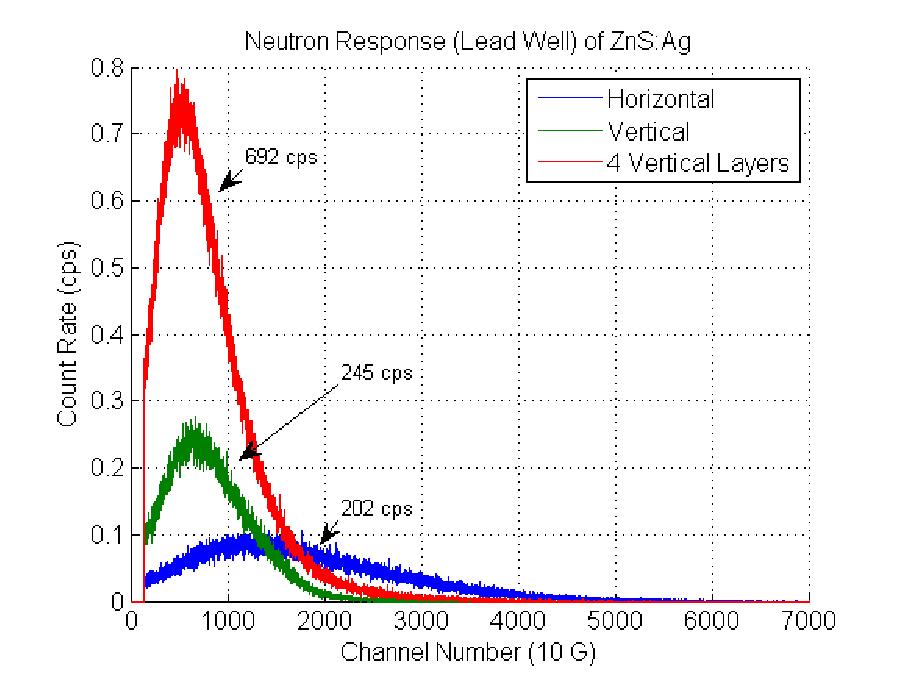
\includegraphics[height=0.6\textheight]{images/EJ426HD_Multi_NeutronComparison.eps}
		\small \caption{Neutron Spectra of EJ426HD2}
	\end{figure}
\end{frame}
%%%%%%%%%%%%%%%%%%%%%%%%%%%%%%%%%%%%%%%%%%%%%%%%%%%%%%%%%%%%%%%%%%%%%%%%%%%%%%%
\begin{frame}{Effects of Layering III}
\dots with only a minimal increase in the gamma response!
\begin{columns}[onlytextwidth]
\begin{column}{0.45\textwidth}
	\tiny
	\begin{figure}
		\centering
		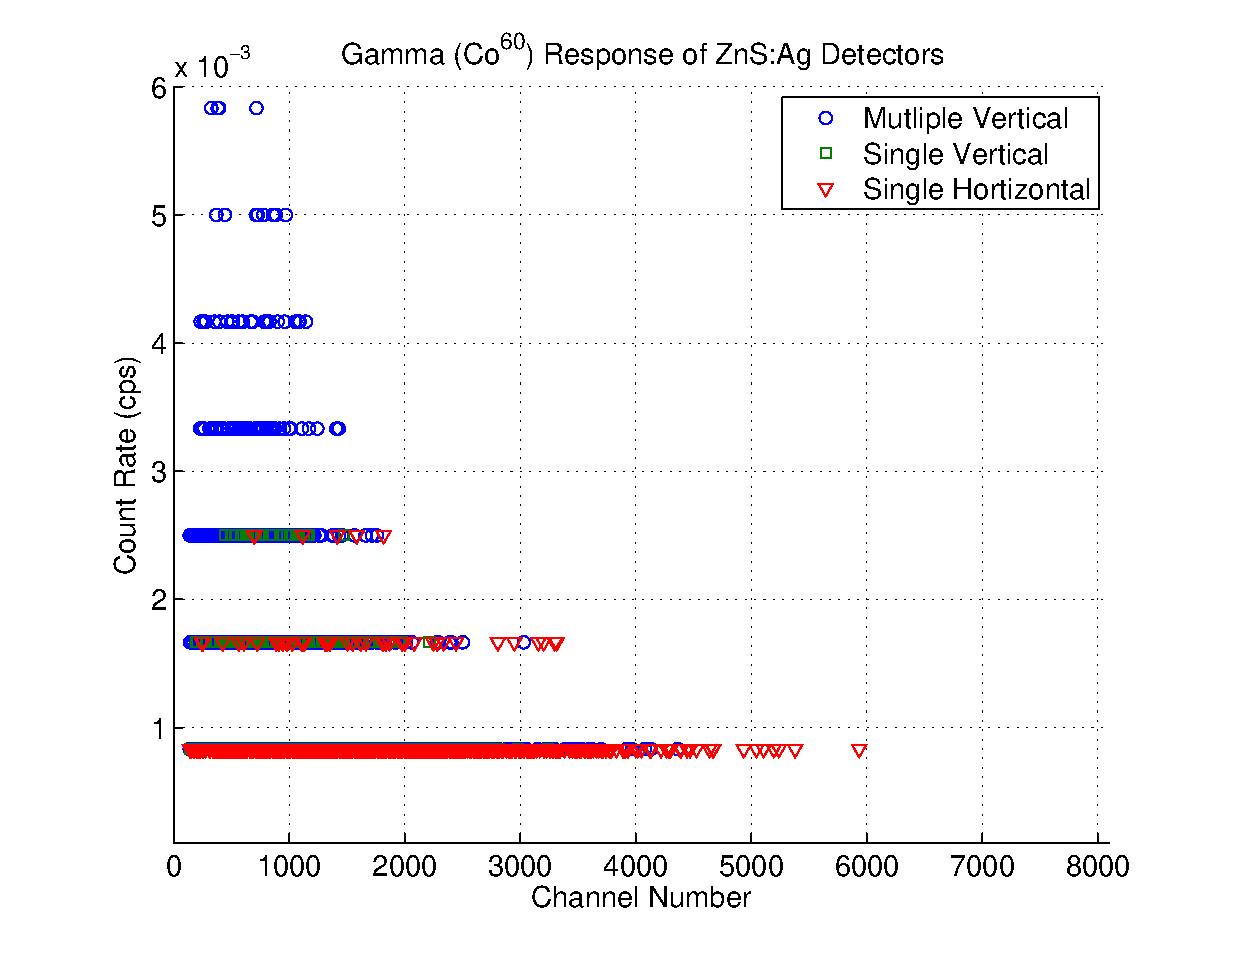
\includegraphics[width=\textwidth]{images/EJ426HD_Multi_GammaComparison.eps}
		\caption{Gamma Spectra of EJ426HD2}
	\end{figure}
\end{column}
\begin{column}{0.45\textwidth}
	\tiny
	\begin{figure}
		\centering
		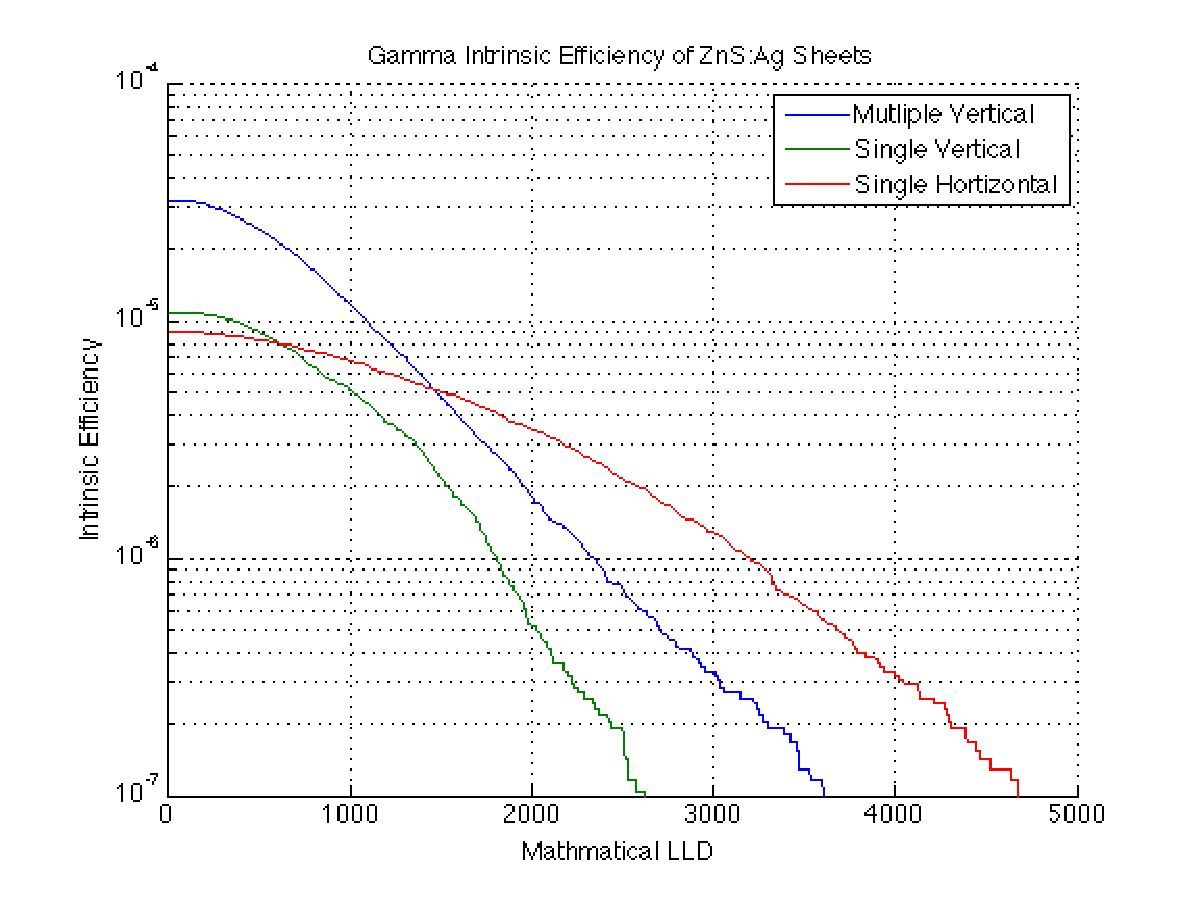
\includegraphics[width=\textwidth]{images/EJ426HD_Multi_GammaIntEff.eps}
		\caption{Gamma Intrinsic Efficiency of EJ426-HD2}
\end{figure}
\end{column}
\end{columns}
\end{frame}
%%%%%%%%%%%%%%%%%%%%%%%%%%%%%%%%%%%%%%%%%%%%%%%%%%%%%%%%%%%%%%%%%%%%%%%%%%%%%%%
\begin{frame}{Multi Film Model}
\begin{columns}[onlytextwidth]
\begin{column}{0.45\textwidth}
\small
120 50$\mu$m PS Films simulated
	\tiny
	\begin{figure}
		\centering
		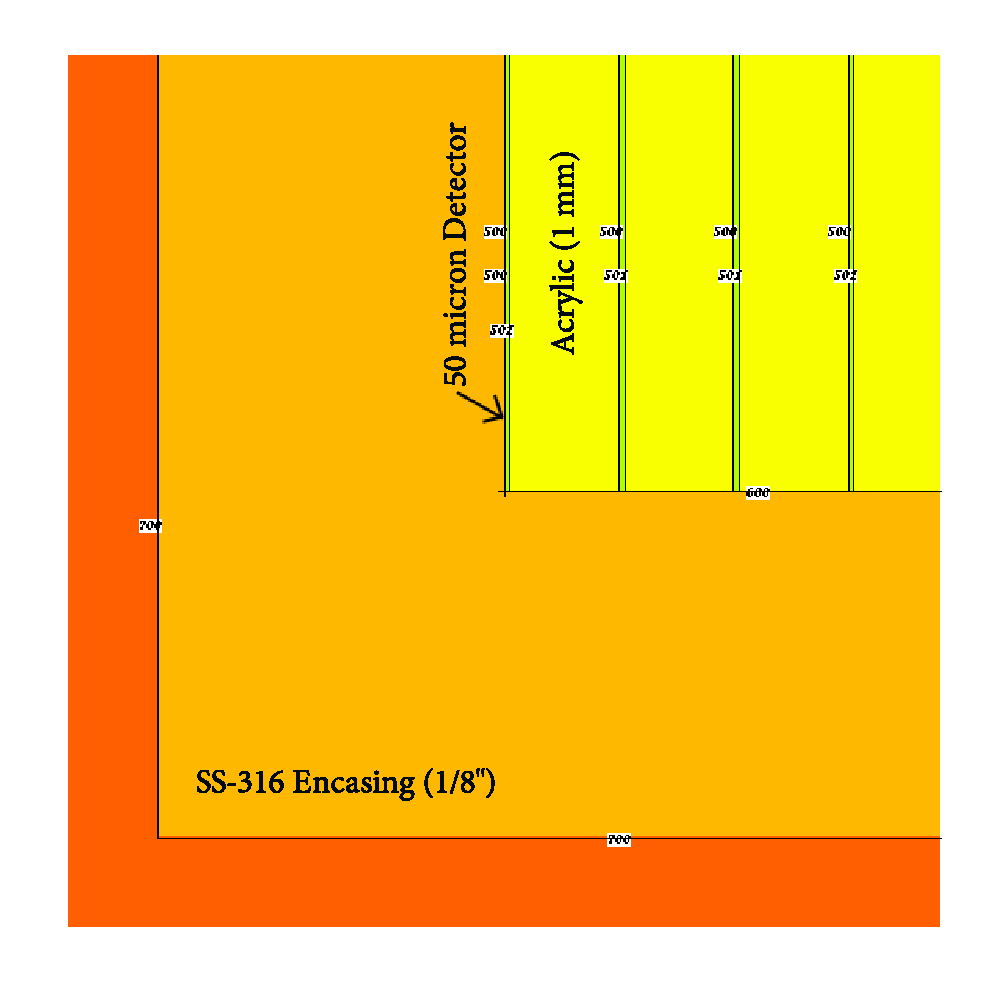
\includegraphics[width=\textwidth]{images/Multi_120Layers.eps}
		\caption{Simulated RPM8 Detector (120 layers)}
	\end{figure}
\end{column}
\begin{column}{0.45\textwidth}
	\tiny
	\begin{figure}
		\centering
		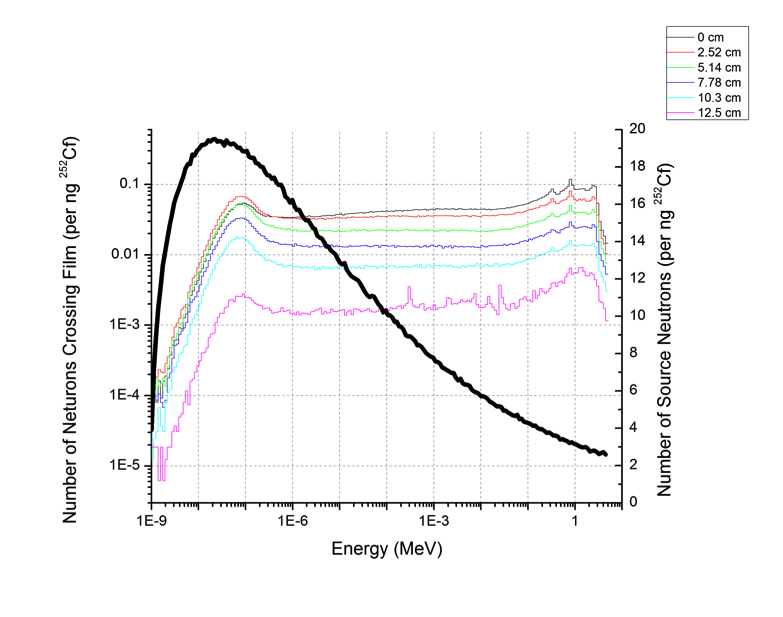
\includegraphics[width=\textwidth]{images/Spectra_Layered.eps}
		\caption{Source and Incident Spectra}
	\end{figure}
\end{column}
\end{columns}
\end{frame}
%%%%%%%%%%%%%%%%%%%%%%%%%%%%%%%%%%%%%%%%%%%%%%%%%%%%%%%%%%%%%%%%%%%%%%%%%%%%%%%
\begin{frame}{Minimum Number of Films}
	\small
	Minimum number of films needed was calculated
	\tiny
	\begin{itemize}
		\item 70 for LiF ZnS:Ag
		\item 85 for PEN
		\item 120 for PS
	\end{itemize}
	\tiny
	\begin{figure}
		\centering
		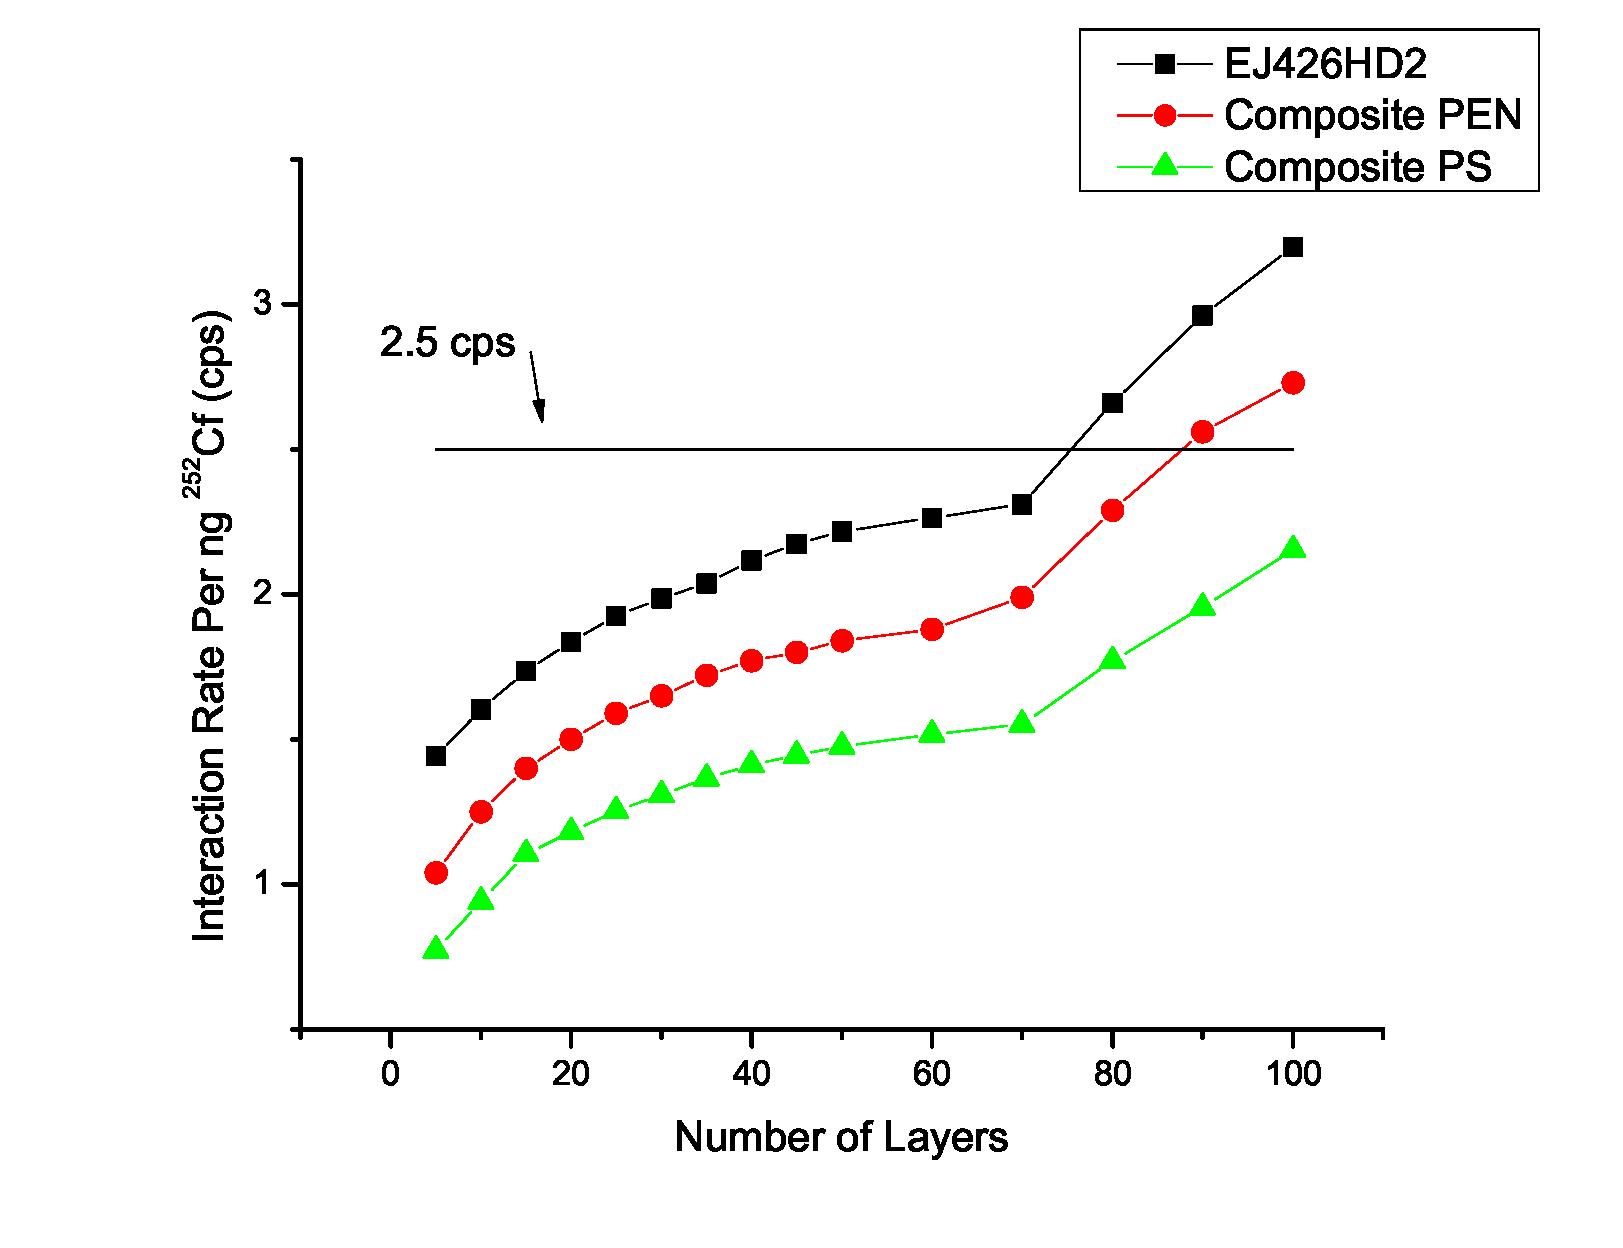
\includegraphics[height=0.6\textheight]{images/OptimalDetectorSize.eps}
		\tiny \caption{Minimum Required Layers}
	\end{figure}
\end{frame}
%%%%%%%%%%%%%%%%%%%%%%%%%%%%%%%%%%%%%%%%%%%%%%%%%%%%%%%%%%%%%%%%%%%%%%%%%%%%%%%
